\documentclass[a4paper,12pt]{article}

%---------------------------------------------------------------------------
% PACKAGES
%---------------------------------------------------------------------------
\usepackage[utf8]{inputenc}
\usepackage[T1]{fontenc}
\usepackage{graphicx}
\usepackage{xcolor}
\usepackage{geometry}
\usepackage{tikz}
\usetikzlibrary{calc}
\usepackage{footmisc}
\usepackage{fancyhdr}
\usepackage{lmodern}
\usepackage{parskip}
\usepackage{background}
\usepackage{array}

%---------------------------------------------------------------------------
% PAGE GEOMETRY & BORDER
%---------------------------------------------------------------------------
\geometry{
left=1in,
right=1in,
top=1in,
bottom=1in
}

\definecolor{mcrred}{HTML}{990000}

\newcommand{\drawborder}{

\begin{tikzpicture}[overlay,remember picture]
\draw[line width=2pt, color=mcrred]
($(current page.north west)+(0.5in,-0.5in)$)
rectangle
($(current page.south east)+(-0.5in,0.5in)$);
\end{tikzpicture}
}

\long\def\symbolfootnotetext[#1]#2{%
\begingroup%
\def\thefootnote{\fnsymbol{footnote}}%
\footnotetext[#1]{#2}%
\endgroup
}

% Symbol footnote settings
\renewcommand{\thefootnote}{\fnsymbol{footnote}}
\renewcommand{\footnotesize}{\color{mcrred}\large}
\makeatletter
\renewcommand\@makefntext[1]{%
\noindent
\makebox[1.8em][r]{\textcolor{mcrred}{\@makefnmark}}#1%
}
\makeatother

\begin{document}
\thispagestyle{empty}

\backgroundsetup{
scale=3,
color=black,
opacity=0.5,
angle=0,
position=current page.center,
contents={%
\IfFileExists{winter_ghibli_background.png}{%
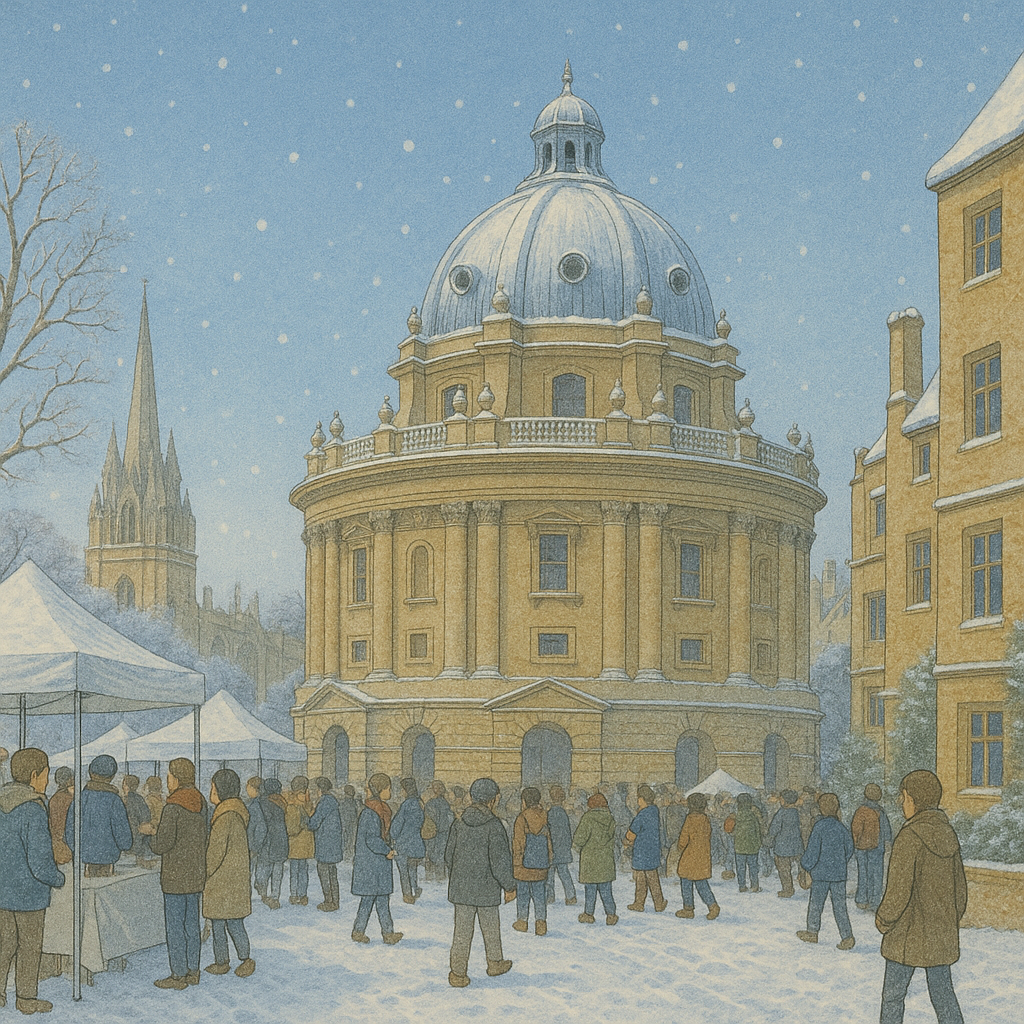
\includegraphics[width=0.63\textwidth]{winter_ghibli_background.png}%
}{}%
}
}

\drawborder

% OPTIONAL vertical centring
\vspace*{\fill}

\begin{center}

\IfFileExists{mansfield_crest.pdf}{%
  
\includegraphics[width=2cm]{mansfield_crest.pdf}%
}{%
  % Built-in fallback used only when the crest file is unavailable.
  
\begin{tikzpicture}
    \draw[line width=1.2pt, color=mcrred] (0,0) circle (0.95cm);
    \node[color=mcrred, font=\bfseries\fontsize{24pt}{24pt}\selectfont] at (0,0) {M};
  \end{tikzpicture}%
}\\[1em]

{\fontsize{22pt}{22pt}\selectfont \textbf{MANSFIELD MCR FRESHERS' WEEK}}\\
{\Large \textit{Michaelmas 2026}}

\vspace{1.2em}

% Retain the column proportions from the 2025 flyer.
\newlength{\colA}\setlength{\colA}{5.5cm}
\newlength{\colB}\setlength{\colB}{9.5cm}

{\color{mcrred}\bfseries\Large EVENTS}\\
\vspace{0.7cm}

\begin{tabular}{@{}p{\colA} >{\raggedleft\arraybackslash}p{\colB}@{}}

\multicolumn{2}{@{}l}{\color{mcrred}\bfseries Sunday, 4 Oct}\\[0.2em]
  & Welcome Tea \hspace{0.5em} 14:00 \\[0.45em]

\multicolumn{2}{@{}l}{\color{mcrred}\bfseries Monday, 5 Oct}\\[0.2em]
  & Group Morning Run \hspace{0.5em} 09:00 \\
  & Oxford Tour \hspace{0.5em} 15:00 \\
  & Sip \& Paint Night \hspace{0.5em} 19:00 \\[0.45em]

\multicolumn{2}{@{}l}{\color{mcrred}\bfseries Tuesday, 6 Oct}\\[0.2em]
  & Oxford Union Tour \hspace{0.5em} 14:00 \\
  & LGBTQ+ Boardgames Night \hspace{0.5em} 19:00 \\[0.45em]

\multicolumn{2}{@{}l}{\color{mcrred}\bfseries Wednesday, 7 Oct}\\[0.2em]
  & College Induction \hspace{0.5em} 09:30 \\
  & \textbf{University} Freshers' Fair \hspace{0.5em} 12:00 \\
  & College EDI Session \hspace{0.5em} 15:30 \\
  & Pub Crawl Night \hspace{0.5em} 19:00 \\[0.45em]

\multicolumn{2}{@{}l}{\color{mcrred}\bfseries Thursday, 8 Oct}\\[0.2em]
  & \textbf{Mansfield} College Freshers' Fair \hspace{0.5em} 10:00 \\
  & Table Tennis Tournament (JCR) \hspace{0.5em} 18:15 \\
  & Freshers' Wine \& Cheese \hspace{0.5em} 19:00 \\[0.45em]

\multicolumn{2}{@{}l}{\color{mcrred}\bfseries Friday, 9 Oct}\\[0.2em]
  & Freshers' Welcome Lunch \hspace{0.5em} 13:00 \\
  & Football Match \hspace{0.5em} 17:00 \\
  & MCR Karaoke Night \hspace{0.5em} 19:00 \\[0.45em]

\multicolumn{2}{@{}l}{\color{mcrred}\bfseries Saturday, 10 Oct}\\[0.2em]
  & MCR Rowing Taster Event \hspace{0.5em} 09:00 \\
  & Picnic at the Park (with LMH) \hspace{0.5em} 12:30 \\[0.45em]

\multicolumn{2}{@{}l}{\color{mcrred}\bfseries Sunday, 11 Oct}\\[0.2em]
  & Sunday MCR Welfare Brunch \hspace{0.5em} 12:30 \\
  & MCR Movie \& Pizza Night \hspace{0.5em} 18:00 \\

\end{tabular}

\end{center}

\vspace*{\fill}

\end{document}